''As the finale of this book, I would like to go over a brief showcase of using the Octalysis Framework to design a project experience from scratch.''

\subsection{The Octalysis Strategy Dashboard}
\begin{itemize}
    \item ''At the beginning of every gamification campaign, the first thing I do is to define five items:
    \begin{enumerate}
        \item Business Metrics, which lead to Game Objective
        \item Users, which lead to Players
        \item Desired Actions, which lead to Win-States
        \item Feedback Mechanics, which lead to Triggers
        \item Incentives, which lead to Rewards
    \end{enumerate}
    \begin{center}
        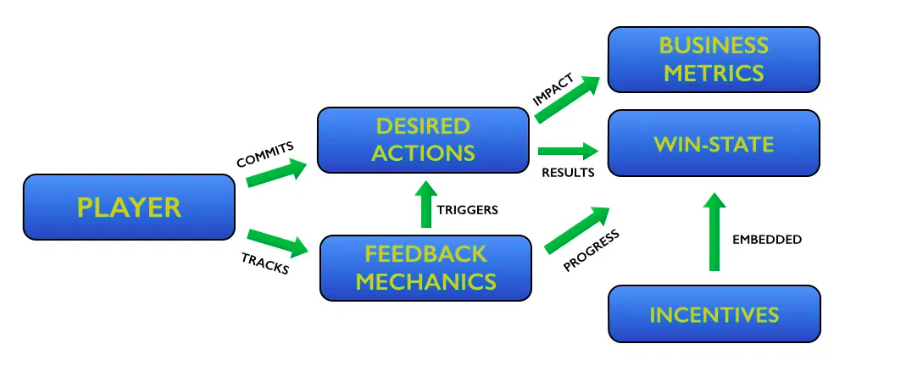
\includegraphics[width=0.6\textwidth]{images/Octalysis_strategy_dashboard.png}
    \end{center}
    These come together to form the Octalysis Strategy Dashboard. Without understanding the business metrics, the users, and the desired actions, it is very difficult to see how effective a gamified design fulfills its objective.''
\end{itemize}

\subsection{Define Business Metrics}
\begin{itemize}
    \item The list that comes from defining the business metrics, ordered by the importance, ''is based on quantifiable metrics for what creates a successful website, and less on my social and personal aspirations. Also, the ones on top are final metrics that would make a project successful, while the ones on the bottom are more of a ''means-to-an-end'' type of metrics.''
    \item ''On every interface, you will realize that you can improve many different Business Metrics, but you can only optimize for one Business Metric with the limited real-estate and user attention span. As a rule of thumb, the question to ask is, if my top three Business Metrics are doing amazingly well, while the other Business Metrics are doing modestly, would this project still be successful.''
    \item ''The Business Metrics then become the Game Objective. If these quantifiable numbers go up, then the gamification campaign is successful. If these metrics do not go up, then the gamification campaign is a failure.''
\end{itemize}

\subsection{Define user Types}
\begin{itemize}
    \item ''The next step is to define who are my target Users, which ultimately become Players in the system if the gamified designs work.''
\end{itemize}

\subsection{Define Desired Actions}
\begin{itemize}
    \item ''The next step is to define the Desired Actions for the Users, which become Win-States once they commit to the actions. This is where we lay out all the little actions and steps that we want users to take in chronological order as part of a player journey.''
    \item \textbf{Discovery Phase Desired Actions}
    \item \textbf{Onboarding Phase Desired Actions}
    \item \textbf{Scaffolding Phase Desired Actions}
\end{itemize}

\subsection{Endgame Phase Desired Actions}
\begin{itemize}
    \item ''Every designed element needs to motivate users towards these Desired Actions. If it does not, the element is a distraction and should be thrown away. Every Desired Action, when committed, leads to a Win-State.''
\end{itemize}

\subsection{Define Feedback Mechanics}
\begin{itemize}
    \item ''Feedback Mechanics are information delivery mechanisms that communicate to the user that their actions are meaningful, It allows them to track their progress towards the Win-State, feel the urgency of time, understand the unpredictable nature of the experience, and more. All Feedback Mechanics should become Triggers that promote the Desired Actions further, or else it should not be there.''
    \item ''The first step to understand possible Feedback Mechanics is to define mediums of interaction and communication. These are all the places I am able to actually plant these Feedback Mechanics as well as Triggers.''
    \item ''The second step is to figure out what Feedback Mechanics I can insert into the site. This is what most people think about when they think ''Gamification Design.'' These are the elements that allow communication of the 8 Core Drives that motivate behavior.''
\end{itemize}

\subsection{Incentives and Reward}
\begin{itemize}
    \item ''The last item to define in the Octalysis Strategy Dashboard is Rewards, which is what the experience designer can give users when they commit the Desired Actions and arrive at the Win-State.''
\end{itemize}

\subsection{Level 1 Octalysis Ideation Process}
\begin{itemize}
    \item ''Once the Octalysis Strategy Dashboard is fully defined, the next step is to go through the 8 Core Drives and come up with new ideas that appeal to people's 8 Core Drives toward the Desired Actions.''
\end{itemize}

\subsection{Repeating the Octalysis Process}
\begin{itemize}
    \item ''Once you go through the 8 Core Drives, don't stop there. Do it again. More sophisticated ideas will often flow out.''
\end{itemize}

\subsection{Summary of Level 1 Octalysis in Action}
\begin{itemize}
    \item ''When designing, it's great when lots of ideas go into the top of a brainstorming funnel. However, it is usually a bad sign when lots of ideas come out of the funnel towards implementation because it shows a lack of focus. Most companies can only implement a subset of the creative ideas in a timely manner.''
\end{itemize}

